% This is "sig-alternate.tex" V2.0 May 2012
% This file should be compiled with V2.5 of "sig-alternate.cls" May 2012
%
% This example file demonstrates the use of the 'sig-alternate.cls'
% V2.5 LaTeX2e document class file. It is for those submitting
% articles to ACM Conference Proceedings WHO DO NOT WISH TO
% STRICTLY ADHERE TO THE SIGS (PUBS-BOARD-ENDORSED) STYLE.
% The 'sig-alternate.cls' file will produce a similar-looking,
% albeit, 'tighter' paper resulting in, invariably, fewer pages.
%
% ----------------------------------------------------------------------------------------------------------------
% This .tex file (and associated .cls V2.5) produces:
%       1) The Permission Statement
%       2) The Conference (location) Info information
%       3) The Copyright Line with ACM data
%       4) NO page numbers
%
% as against the acm_proc_article-sp.cls file which
% DOES NOT produce 1) thru' 3) above.
%
% Using 'sig-alternate.cls' you have control, however, from within
% the source .tex file, over both the CopyrightYear
% (defaulted to 200X) and the ACM Copyright Data
% (defaulted to X-XXXXX-XX-X/XX/XX).
% e.g.
% \CopyrightYear{2007} will cause 2007 to appear in the copyright line.
% \crdata{0-12345-67-8/90/12} will cause 0-12345-67-8/90/12 to appear in the copyright line.
%
% ---------------------------------------------------------------------------------------------------------------
% This .tex source is an example which *does* use
% the .bib file (from which the .bbl file % is produced).
% REMEMBER HOWEVER: After having produced the .bbl file,
% and prior to final submission, you *NEED* to 'insert'
% your .bbl file into your source .tex file so as to provide
% ONE 'self-contained' source file.
%
% ================= IF YOU HAVE QUESTIONS =======================
% Questions regarding the SIGS styles, SIGS policies and
% procedures, Conferences etc. should be sent to
% Adrienne Griscti (griscti@acm.org)
%
% Technical questions _only_ to
% Gerald Murray (murray@hq.acm.org)
% ===============================================================
%
% For tracking purposes - this is V2.0 - May 2012

\documentclass{sig-alternate}

\usepackage{algorithm}
\usepackage{algpseudocode}
\begin{document}
%
% --- Author Metadata here ---
\conferenceinfo{CS 760}{'14, Madison WI, USA}
\CopyrightYear{2014} % Allows default copyright year (20XX) to be over-ridden - IF NEED BE.
%\crdata{0-12345-67-8/90/01}  % Allows default copyright data (0-89791-88-6/97/05) to be over-ridden - IF NEED BE.
% --- End of Author Metadata ---

\title{BoostEM}
\subtitle{A Semi-Supervised Ensemble Method}
%
% You need the command \numberofauthors to handle the 'placement
% and alignment' of the authors beneath the title.
%
% For aesthetic reasons, we recommend 'three authors at a time'
% i.e. three 'name/affiliation blocks' be placed beneath the title.
%
% NOTE: You are NOT restricted in how many 'rows' of
% "name/affiliations" may appear. We just ask that you restrict
% the number of 'columns' to three.
%
% Because of the available 'opening page real-estate'
% we ask you to refrain from putting more than six authors
% (two rows with three columns) beneath the article title.
% More than six makes the first-page appear very cluttered indeed.
%
% Use the \alignauthor commands to handle the names
% and affiliations for an 'aesthetic maximum' of six authors.
% Add names, affiliations, addresses for
% the seventh etc. author(s) as the argument for the
% \additionalauthors command.
% These 'additional authors' will be output/set for you
% without further effort on your part as the last section in
% the body of your article BEFORE References or any Appendices.

\numberofauthors{2} %  in this sample file, there are a *total*
% of EIGHT authors. SIX appear on the 'first-page' (for formatting
% reasons) and the remaining two appear in the \additionalauthors section.
%
\author{
% You can go ahead and credit any number of authors here,
% e.g. one 'row of three' or two rows (consisting of one row of three
% and a second row of one, two or three).
%
% The command \alignauthor (no curly braces needed) should
% precede each author name, affiliation/snail-mail address and
% e-mail address. Additionally, tag each line of
% affiliation/address with \affaddr, and tag the
% e-mail address with \email.
%
% 1st. author
\alignauthor
Zach Welch\\
       \affaddr{UW--Madison}\\
       \email{zwelch@cs.wisc.edu}
% 2nd. author
\alignauthor
Steven Johnson\\
       \affaddr{UW--Madison}\\
       \email{sjj@cs.wisc.edu}
}
\date{May 12, 2014}
% Just remember to make sure that the TOTAL number of authors
% is the number that will appear on the first page PLUS the
% number that will appear in the \additionalauthors section.

\maketitle
\begin{abstract}
We introduce BoostEM, a semi-supervised ensemble method which combines the benefits of using an ensemble method like Boosting with the benefits of using unlabeled data.  BoostEM is intended for learning settings with an abundance of unlabeled data. By using the weights from each iteration of AdaBoost as weights in Expectation Maximization, BoostEM can refocus its underlying model of the data distribution to place more emphasis on difficult to classify instances. BoostEM combines AdaBoost and using fractional count data via Expectation Maximization, and with specific parameters BoostEM can reduce to either algorithm. BoostEM outperforms the traditional AdaBoost and learning with fractional data from using Expectation Maximization across a variety of base learners and data sets. Additionally, we have found that BoostEM performs comparably to only using its base learner (ID3 decision trees and Naive Bayes were tested) with one fifth of the labeled data.  
\end{abstract}

% A category with the (minimum) three required fields
\section{Introduction}

In many machine learning classification problems, labels are difficult to obtain while unlabeled data are abundant. Examples of such situations are labeling x-rays as benign or malignant, tweets as instances of bullying, news articles as interesting to a given reader, or whether a photograph contains a given object. Because of this scarcity of labeled instances, using semi-supervised learning techniques, such as Expectation Maximization, to combine unlabeled and labeled data into an integrated model is a good idea to potentially improve learner accuracy and reduce human labour.

This paper describes the development and evaluation of a semi-supervised learning algorithm, BoostEM, which combines the benefits of an ensemble method like Boosting with the benefits of using unlabeled data. The next section provides background information on Boosting and Expectation Maximization. The following section describes related work in semi-supervised learning and ensemble methods. This section is followed by the details of the BoostEM algorithm and an experimental evaluation of our implementation. We then present the results of our evaluation and discuss our findings and their implications.

\section{Background}
\subsection{AdaBoost}
Boosting is an ensemble method which uses a set of learners trained on weighted versions of a training set. A popular boosting algorithm is known as AdaBoost (short for Adaptive Boost) originally detailed in ~\cite{Freund:1997:DGO:261540.261549}.  AdaBoost works by giving each training set instance a weight $W_{i}$; initially all weights are equal. Over some number of iterations, AdaBoost trains a base learner (ID3 decision trees, Naive Bayes, etc.) proportionally to the weights of each instance. The weighted training set error $\epsilon$ of this base learner is calculated and if more than half of the instances by weight were incorrect AdaBoost quits.  Otherwise, $\beta=\frac{\epsilon}{1-\epsilon}$ is multiplicatively applied to all of the correctly guessed instances, decreasing their weights. This means that in the next iteration, incorrectly classified instances will be given more importance.  AdaBoost then essentially drives up the importance of difficult to classify training set instances in an effort to correctly learn them. To classify a new instance $\bf{x}$, with base learners $H_{1} \dots H_{T}$  $\arg \max_{y} \sum_{i=1}^{T}\bigg(\log(\frac{1}{\beta_{t}})\bigg) \delta(H_{t}(\bf{x}),y)$ where $\delta(a,b)$ is the indicator function.

Empirical studies~\cite{dietterich1997machine} have shown that in a large majority of instances AdaBoost improves accuracy over the base learner. There are a few occasions, however, where using Boosting can hurt performance. This implies that when using AdaBoost, one should take care to compare results from the combined learner to those from a base learner.

\subsection{Expectation Maximization}
Expectation is an iterative algorithm which uses the values of existing, complete data points to compute the maximum likelihood estimate for missing values for other, incomplete data. Expectation Maximization was originally introduced in~\cite{Dempster77maximumlikelihood} and produces a probabalistic distribution of the possible values of missing data given fully labeled data. Expectation maximization is not itself a learning algorithm in the way ID3 or Naive Bayes are, though it is often used with unlabeled data.

In the context of semi-supervised learning, there is a set of labeled input data and a potentially much larger set of unlabeled data and for each unlabeled instance u, EM can provide a probability for each label. As originally described in~\cite{nigam2000text}, these probabilities can be used as fractional instances of labeled data, making the input training set much bigger and diverse and potentially giving a better approximation of the distribution of labels to the learner. In many cases, performance can be drastically improved by using these fractional counts. Even if the learner in question cannot handle a fractional amount of a data point (and many cannot), this can be avoided by sampling a much larger training set, with each instance existing proportional to its fractional count. In this way using fractional data can be roughly approximated.

Expectation maximization is a general approach and can be augmented to suit a variety of settings and assumptions. For instance, in our implementation of BoostEM, we assume the data is well modeled by a Gaussian mixture model and the instances have weights associated with them.
     
\section{Related Work}
Semi-supervised learning and Ensemble Methods are both extremely well studied research areas; for surveys of semi-supervised learning and ensemble methods, we direct the reader to ~\cite{zhu05survey} and~\cite{dietterichl2002ensemble} respectively. 

Additionally, combining unlabeled instances with ensemble methods is not a new idea. Blum and Mitchell's well known Co-training algorithm~\cite{blum1998combining} uses two learners trained on subsets of data to improve performance with unlabeled data. By using the confidence of a prediction from one learner to expand the labeled training set for the other learner, overall performance can be drastically improved over using only the explicitly labeled data. The independence requirements for the features of the two learners are quite strong. 

In~\cite{li2007improve}, the idea of using two learners with independent sets of features was extended and combined with the popular ensemble method of random forests~\cite{breiman2001random} to create the Co-forest algorithm. Because Co-forests use larger numbers of classifiers instead of two, it is very unlikely the strong independence requirments from Co-training will apply, and so they are relaxed.

Many semi-supervised ensemble methods, including BoostEM, use the AdaBoost algorithm due to its performance increases. These algorithms differ in how they assign ``effective'' class labels to the large amount of unlabeled data.  BoostEM uses weighted Expectation Maximization to infer a probability distribution amongst labels. In~\cite{bennett2002exploiting}, the ASSEMBLE algorithm generates provisional classes for unlabeled using Suport Vector Machine esque large margins on the weighted labeled instances.  Though we have run no tests, we suspect that if our soft EM algorithm were replaced with a hard EM algorithm, BoostEM would produce similar behavior to ASSEMBLE. Margin assumptions are similarly used in~\cite{grandvalet2001semi}

In~\cite{kumar2009semiboost}, the SemiBoost framework is discussed. SemiBoost is a general framework for integrating many graph and cluster based semi-supervised learning methods in an iterative Boosting algorithm.  SemiBoost is very general and it is likely that implementations like ASSEMBLE and BoostEM are realizations of the SemiBoost Framework.  



\section{BoostEM}
The main insight of BoostEM is observing that Boost and Expectation Maximization both attempt to improve the current iteration's results by using information from the previous iteration; BoostEM simply couples the results of the two algorithms together to improve results.  BoostEM uses a weighted EM algorithm, and these weights are identical to the weights used in the Boost algorithm.  At its most basic level, BoostEM simply runs a weighted Expectation Maximization on the unlabeled instances, and uses the fractional counts to create a weighted training set for some base learner.  The results of this base learner are then used to update the weights, which are then input to EM in the next iteration. 


\begin{algorithm}
\caption{BoostEM}\label{euclid}
\begin{algorithmic}[1]
\State L=Labeled Data
\State U=Unlabeled Data
\State H=Learner
\State T=Number of Boost iterations

\Procedure{BoostEM}{$L,U,H,T$}
\State for $i \in |L|$, $ Wl(i) \gets 1$
\State for $i \in |U|$, $ Wu(i) \gets 1$

\For{$t=1 \dots T$}
\State Normalize $Wu,Wl$
\State get fractional counts $P_{t} \gets EM(L,U,Wl,Wu)$
\State $H_{t} \gets \text{model learned from L, fractional counts of U}$
\State $\epsilon_{t} = \sum_{i=1}^{|L|} Wl_{i}(1-\delta(h_{t}(L_{i}),y_{i}))$
\State $\epsilon_{t} += \sum_{i=1}^{|U|} Wu_{i}(1-\delta(h_{t}(L_{i}),{P_{t,}}_{h_{t}(L_{i})}))$
\State if $|U| > 0$ then $\epsilon /= 2$
\State $\beta_{t} \gets \frac{\epsilon_{t}}{1-\epsilon_{t}}$
\State for $i,h_{t}(L_{i} = y_{i}) \in |L| Wl(i) \gets Wl(i)*\beta_{t}$
\State for $i \in |U|$, $Wl(i) \gets Wu(i)*\beta_{t}$

\EndFor
\State \textbf{return} $\arg \max_{y} \sum_{i=1}^{T}\bigg(\log(\frac{1}{\beta_{t}})\bigg) \delta(H_{t}(\bf{x}),y)$
\EndProcedure
\end{algorithmic}
\end{algorithm}

 Using an unweighted version of Expectation Maximization is possible, but since the training set data itself is not changing, the fractional counts will not change from iteration to iteration. By combining the AdaBoost weights with the EM algorithm, BoostEM is able to alter the distribution and get an updated set of fractional counts in each iteration of BoostEM.   By using a weighted EM, we can place more emphasis on the instances our learner incorrectly classifies in the Gaussian distribution of instances we assume. Or more correctly, since there is no ground truth to the unlabeled instances, we can penalize every prediction from learner $H$ on unlabeled instance $x$ by $1-p(H(x))$, where $p$ is the distribution of labels from EM.  In this way, the learner penalizes unexpected labels (ones with small probability) more than expected ones.

Notice as well that using Expectation Maximization for fractional counts and AdaBoost can be recovered from BoostEM by setting certain inputs and parameters.  Setting the number of boosting iterations to 1 is equivalent to EM, while inputting no unlabeled instances reduces to traditional labeled Boosting.    
    
\section{Evaluation}
We implemented the BoostEM algorithm in \textsc{python} and evaluated its accuracy against a number of other algorithms using two learners and a variety of parameter settings  as described below.


\subsection{Data sets}

We evaluated the performance of our algorithm on four data sets from the UCI Machine Learning Repository: Breast Cancer Wisconsin (Diagnostic), which classifies digitized images of breast mass as benign or malignant; Parkinsons, which classifies biomedical voice measurements from patients as healthy or Parkinson's; Banknote Authentication, which classifies pictures of currency as genuine or foraged; and Vertebral Column, which classifies biomedical data from patients as either normal or abnormal vertebral column. Each dataset is for a binary classification task, and each attribute is real-valued. For each dataset, the number of attributes ranges from 5 to 32 and the number of instances ranges from 197 to 1372. 

\subsection{Implementation Details}
In our testing, we only attempt to test BoostEM in classification.  Because of this, we choose to use a Gaussian mixture model as the underlying model for data. Given a classification label, we assume the conditional distribution of the data to be gaussian distributed. One of the benefits of assuming an underlying distribution in Expectation Maximization is that it allows us to use both labeled data and a potentially much larger amount of unlabeled data in the maximization step. This choice may not be appropriate for all data sets; we chose Gaussian mixture models because many data sets can be roughly approximated by such a model.  A different underlying model which provides a better fit to the data will produce likely produce better results.  An overview of EM and Gaussian Mixture Models can be found in ~\cite{zhu2009introduction}.

\subsection{Benchmark Algorithms}

We used five other algorithms for comparison to BoostEM to evaluate its performance. The following lists the algorithms' abbreviations as used in the graphs and discussion section and describes them.

\begin{enumerate}
\item \textbf{BoostEM}: our implementation of the BoostEM algorithm
\item \textbf{FullBoost}: applying the AdaBoost algorithm to the fully labeled dataset
\item \textbf{justBoost} applying the AdaBoost algorithm to the fraction of the labeled dataset
\item \textbf{justEM} applying Expectation Maximization to the fraction of the labeled dataset
\item \textbf{full\{Algorithm A\}} applying A to the fully labeled dataset without Boosting or EM
\item \textbf{just\{Algorithm A\}} applying A to the fraction of the labeled dataset without Boosting or EM
\end{enumerate}

\subsection{Methodology}

We evaluated the aforementioned algorithms manipulating the following parameters.

\begin{enumerate}
\item \textbf{Dataset}: Breast Cancer Wisconsin (Diagnostic), Parkinsons, Banknote Authentication, Vertebral Column
\item \textbf{Base Learner}: ID3 Decision Tree, Naive Bayes
\item \textbf{Fraction of Labeled Instances} 5\%, 20\%
\end{enumerate}

For each combination of these parameters, we averaged the resulting accuracies of five 10-fold cross validation runs. 

\subsection{Results}

In our testing, we varied our results among four datasets, two base learners, and two fractions of labeled data, for a total of sixteen data set/base learner/fraction triples, which we will define as a setting.  

For the Parkinsons dataset, with $20\%$ of the total data being labeled and using an ID3 base learner, BoostEM achieved an average accuracy of 73.54\%, FullBoost 86.94\%, justBoost an accuracy of 33.14\%, fractional counts using EM 68.78\%, fullID3 84.86\%, and justID3 an accuracy of 33.04\% as visualized in Figure~\ref{parkAcc}. With only 5\% of the total training data labeled, BoostEM increased to 74.64\%, justBoost fell to 26.64\%, EM to 60.5\%, and justID3 managed 26.66\%.  FullBoost and fullID3 maintained their values because their inputs were not affected by the change. Using instead the weka implementation of Naive Bayes, at 20\% labeled data, BoostEM's accuracy was 76.52\%, FullBoost had 69.78\%, justBoost curiously managed 74.78\%, EM 68.16\%, FullNB 70.38\%, and JustNB 71.98\%. At 5\% labeled data, BoostEM reached 69.24\%, JustBoost 42.06\%, EM 55.46\%, and JustBoost only 42.34\%.

\begin{figure}
\centering
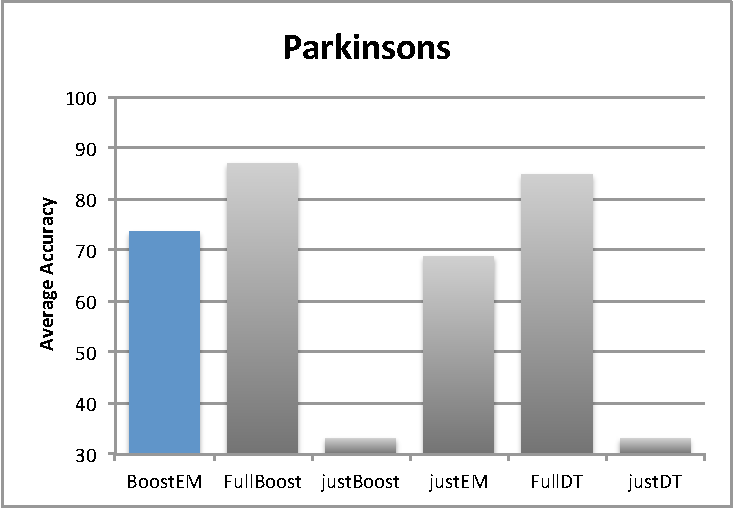
\includegraphics[width=0.35\textwidth]{figures/parkAcc.pdf}
\caption{Average 10 fold cross validation \% accuracy using ID3 on Various algorithms, 20\% labeled data}
\label{parkAcc}
\end{figure}

Using the vertebral column data and shown in Figure~\ref{vertAcc}, 20\% labeled data, and ID3, BoostEM: 75.28\%, FullBoost: 82.4\%, JustBoost: 72.76\%, EM: 73.78\%, FullID3 80.36\%, justID3: 72.2\%.  Using 5\% data, BoostEM: 70.14\%, justBoost: 68.08\%, EM: 64.78\%, justID3: 68.04\%. 
Using Naive Bayes and 20\% labeled data, BoostEM: 78.34\%,FullBoost: 83.46\%, justBoost: 80.04\%, EM: 76.16\%, FullNB 77.88\%, and justNB: 78.02\%. Using instead 5\% labeled data BoostEM: 70.2\%, JustBoost: 78.56\%, EM: 69.44\%, and justNB: 73.56\%.

\begin{figure}
\centering
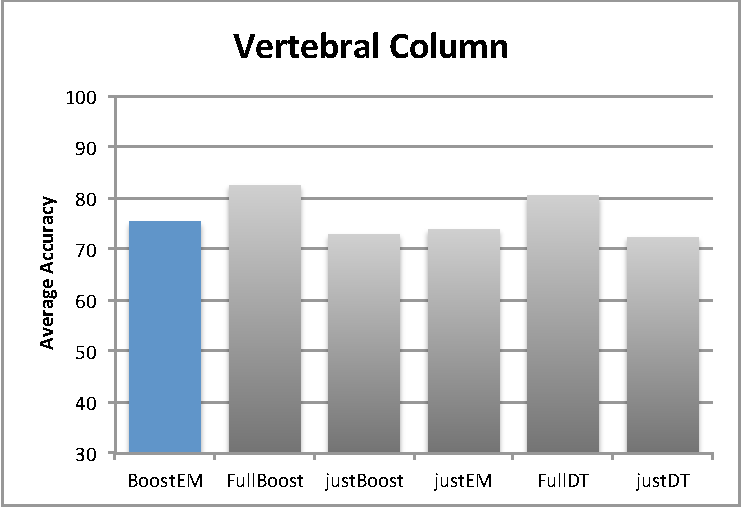
\includegraphics[width=0.35\textwidth]{figures/vertAcc.pdf}
\caption{Average 10 fold cross validation \% accuracy using ID3 on Various algorithms, 20\% labeled data}
\label{vertAcc}
\end{figure}

Banknote authentication data can be found in Figures~\ref{bankAcc} and~\ref{bankAcc5}. At 20\% of the labeled data, BoostEM reaches 98.12\% accuracy, FullBoost is almost perfect with 99.74\%, JustBoost with 98.38\%, EM a much lower 90.9\%, FullID3 a 96.68\%, and justID3 87.46\% accuracy.  With the smaller amount of labeled data, BoostEM averages 94.02\%, JustEM only 66.86\%, EM retains its performance with 88.62\%, and JustID3 a relatively low 62.54\%.
Using NB instead, BoostEM had a test set accuracy of 96.12\%, FullBoost 99.18\%, JustBoost 98.52\%, EM 84.24\%, FullNB 83.86\%, and JustNB 84.38\% accuracy at one fifth labeled data. BoostEM had 93.08\%, JustBoost 95.08\%, EM with 84.64\%, and JustNB 83.32\% using one twentieth of the labeled information.
\begin{figure}[ht!]
\centering
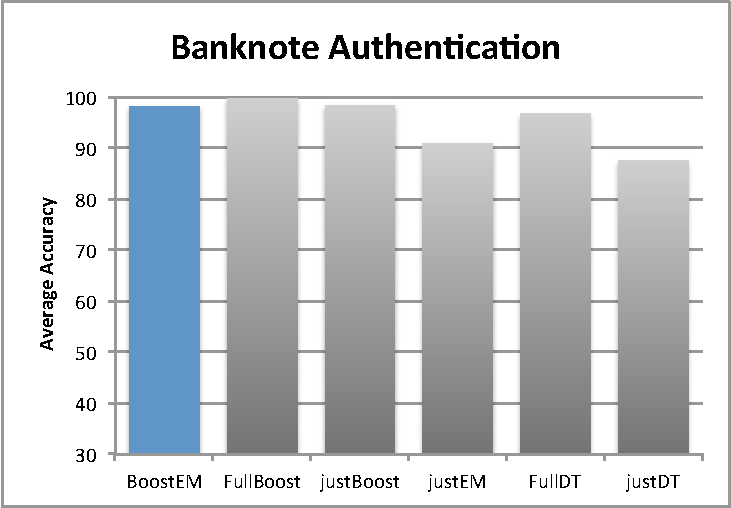
\includegraphics[width=0.35\textwidth]{figures/bankAcc.pdf}
\caption{Average 10 fold cross validation \% accuracy using ID3 on Various algorithms, 20\% labeled data}
\label{bankAcc}
\end{figure}
\begin{figure}
\centering
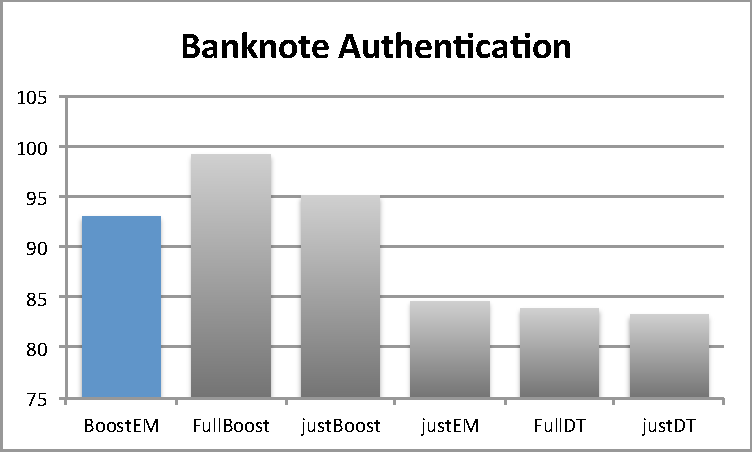
\includegraphics[width=0.35\textwidth]{figures/bankAcc5.pdf}
\caption{Average 10 fold cross validation \% accuracy using Naive Bayes on Various algorithms, 5\% labeled data}
\label{bankAcc5}
\end{figure}



Finally, with the Wisconsin Breast Cancer data, using ID3 and 20\% labeled data, the average accuracies were: BoostEM 93.5\%, FullBoost 95.62\%, justBoost 77.52\%, EM 91.08\%, FullID3 92.7\%, JustID3 78.18\%. At 5\% labeled data the results were: BoostEM 87.78\%, JustBoost 62.96\%, EM 86.24\%, and JustID3 62.96\%.
With Naive Bayes and 20\% labeled data: BoostEM 92.64\%, FullBoost 95.4\%, JustBoost 94.08\%, EM 91.62\%, FullNB 92.6\%, and JustNB 92.48\%. at 5\% labeled data these accuracies were BoostEM 86.86\%, JustBoost 74.78\%, EM 90.66\%, and JustNB 78.32\%.
\begin{figure}[ht!]
\centering
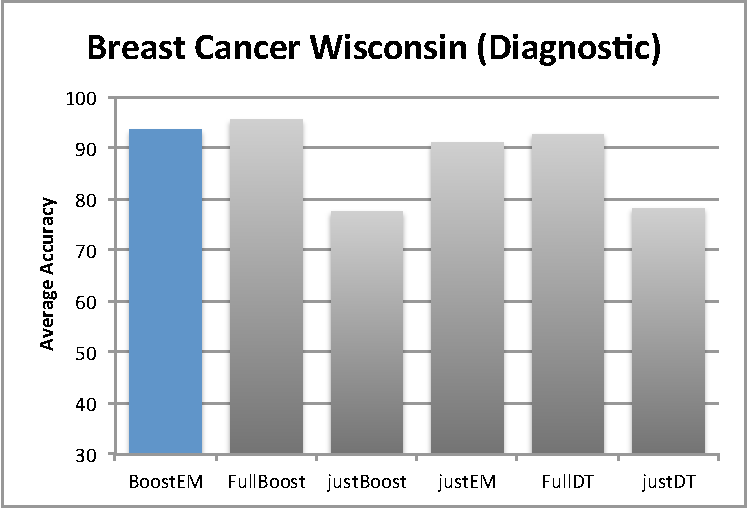
\includegraphics[width=0.35\textwidth]{figures/breaAcc.pdf}
\caption{Average 10 fold cross validation \% accuracy using ID3 on Various algorithms, 20\% labeled data}
\label{breaAcc}
\end{figure}
\begin{figure}[ht!]
\centering
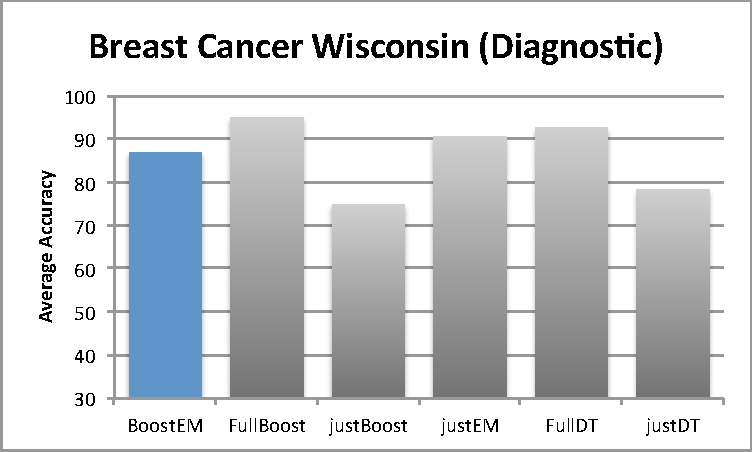
\includegraphics[width=0.35\textwidth]{figures/breaAcc5.pdf}
\caption{Average 10 fold cross validation \% accuracy using Naive Bayes on Various algorithms, 5\% labeled data}
\label{breaAcc5}
\end{figure}
 

\section{Discussion}

\begin{figure}
\centering
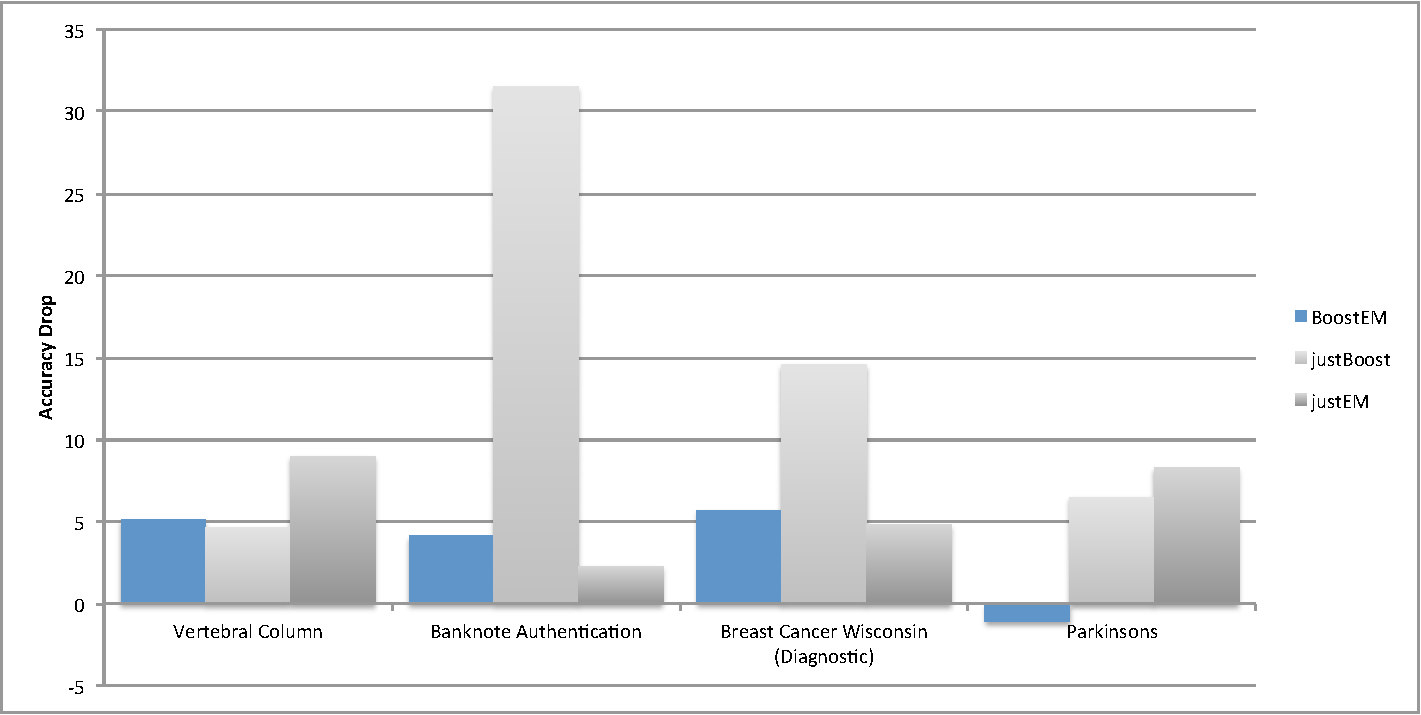
\includegraphics[width=0.35\textwidth]{figures/accDrops.pdf}
\caption{Average decrease in 10 fold cross validation \% accuracy using ID3 from 20\% to 5\% of the data being labeled}
\label{accDrop}
\end{figure}

 Among the six algorithms we ran cross validation for, we expected FullBoost to have the best average performance, JustAlg to
have the worst average performance, and the other four algorithms to perform in between. In general, this intuition was found to be true about FullBoost.
FullBoost was the top performing algorithm in 15 of the 16 settings we tested.
The only algorithm to best it was BoostEM on the parkinsons data set
with 20\% labeled data. JustAlg, however, only performed worse than all other algorithms in 5 settings. JustBoost and EM were each the worst performing algorithm
in 5 settings.

Ideally, BoostEM would in general perform better than both JustBoost and EM since it is a generalization and combination of the two techniques. This is the case, 
with BoostEM improving over both EM and Boost in 9 settings, and performing better than EM in 15 settings, and better than justBoost in 10. In no instances is BoostEM 
the worst performing of the three algorithms.

Somewhat surprisingly, BoostEM with 20\% of the data also outperformed using all the data on the base learner in 6 out of the 8 settings we tested.  This would seem to imply our learner can outperform a traditional base learner while only using one fifth of the labeled data.

BoostEM also performs well when the amount of labeled data is decreased by a large amount (one fourth).  In most cases, BoostEM retains its accuracy better than Boost and comparably to EM.

In general it seems that fluctuations in average accuracy when BoostEM uses a different base learner is mostly due to the base learner in question, as accuracy changes by BoostEM are reflected in accuracy changes using only the base learner.


\section{Conclusions}
We presented BoostEM, a semi-supervised ensemble method.  BoostEM works by combining fractional counts from using the Expectation Maximization algorithm with the AdaBoost ensemble method.  We tested BoostEM on four large datasets from the UCI repository, performing 10-fold cross validation and five random restarts for EM.  We compared using 20\% labeled data to 5\% labeled data, the rest being unlabeled and used ID3 decision trees and Naive Bayes as base learners.  BoostEM was compared to Boosting with 100\% of the data, Boosting with only the percentage of labeled data, performing only Expectation Maximization on the unlabeled data and using the base learner, using the base learner on all the data, and finally using only the subset of unlabeled data with a base learner. We found that in the majority of settings, BoostEM outperforms using only Boosting or only Expectation Maximization. Additionally, we found that across data sets and base learners that BoostEM performs comparably to only using a base learner, but with only one fifth of the labeled data. Since with specific parameters, BoostEM can replicate both AdaBoost and EM, BoostEM can always achieve performance on a data set at least as well as them, and we have shown that in many cases BoostEM can also improve performance.

%ACKNOWLEDGMENTS are optional
\section{Acknowledgments}
Zach would like to thank his cats, who only broke one of his coffee mugs in the course of this project. Steve would like to thank Zhi and Brandi for being in the room while he edited this paper.

\bibliographystyle{abbrv}
\bibliography{paper}  % sigproc.bib is the name of the Bibliography in this case

\end{document}
